
In this subsection, we relate the free energy to the amplitudes between boundary states and present the analytic results. 

We notice that there is only one apparent length scale in these diagrams -- the finite size $L$ for fidelity and imaginary time $\tau$ for the Loschmidt echo. These are the characteristic size of the corner at the tip of the slit. Regulators are necessary in keeping track of the scale dependence, otherwise a dilation transformation can rescale both $L$ and $\tau$ to $1$ and get rid of their dependence. The introduction of regulators is also physically sensible when considering the lattice realization of the systems. 

We thus add small semi-circles around the points where the bcc operators reside, and then apply a series of conformal mapping. 

For the fidelity case, the regulators as well as the conformal mappings are depicted in Fig.~\ref{fig:fidel-map}. 
\begin{figure}[h]
\centering
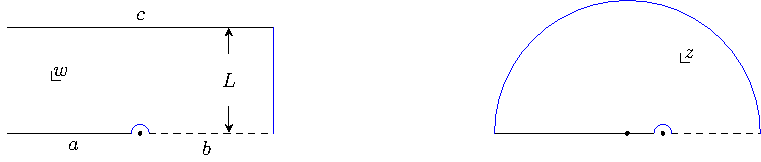
\includegraphics[width=\columnwidth]{fig_fidel-map.pdf}
\caption{Mapping from a strip to the upper half plane $\xi  = \exp( \frac{\pi z}{L} ) $. The two black dots represent possible locations of boundary condition changing (bcc) operators. The dot inside the blue semi-circle is at coordinate $z = 1$, which is the image of the point connecting $a$ and $b$ boundaries. The other dot is at $z = 0$ and corresponds to the connection between $a$ and $c$ boundaries at $- \infty$. To evaluate the diagram, we add the outer blue semi-circle centered at $z = 1$ to be the IR cut-off and map it to the cylinder with $w = \ln(z - 1)$}
\label{fig:fidel-map}
\end{figure}
We add a small blue semi-circle to the folded strip in Fig.~\ref{fig:fidel} as the UV regulator and map it to the upper half plane using $\xi  = \exp( \frac{\pi z}{L} )$. Then both of $z = 0$ and $1$ can host bcc operators. We assume $a = c$ such that there is only one bcc operator on the real axis enclosed by the blue semi-circle at $z = 1$. In order to evaluate this diagram, we add another semi-circle centered at $z = 1$ with radius $R_{\xi}$ (this will introduce a correction as explained in App.~\ref{app:F_correction}), and map it to the cylinder diagram on the right by $w = \ln ( z- 1)$. Finally the cylinder diagram can be viewed as path integral amplitude between the boundary state $b$ and $a$
\begin{equation}
Z_{ab} = \langle a | e^{-\pi H } |b \rangle
\end{equation}

The height of the cylinder is $\pi$. The two end points of the $\epsilon$ radius semi-circle on the $z$ plane are mapped to
\begin{equation}
\exp( \pm \pi \frac{\epsilon}{ L}  ) \sim 1 \pm \pi \frac{\epsilon}{L} .
\end{equation}
The bigger blue semi-circle intersects the real axis at $1 \pm R_{\xi}$. So the width of the cylinder is 
\begin{equation}
\label{eq:fidel_cyd_width}
\ln R_{\xi} - \ln \frac{\pi \epsilon}{L} = \ln L + \text{constant} 
\end{equation}

The Loschmidt echo can be evaluated in the same way. Again, we introduce two semi-circles (blue in Fig.~\ref{fig:H-tau_fold}) as regulators and then perform the conformal transformation shown in Fig.~\ref{fig:H-tau_fold}. From $z$ plane to the $\xi$ plane, we use $\xi = \frac{z}{\tau - z}$ to map the two slits to half of an annulus, which is the same as the fidelity case. With one more conformal mapping $w = \ln \xi$, the diagram becomes the cylinder partition function between the two boundary states. 

The height of the cylinder is still $\pi$ because of folding. In the $\xi$ plane, the two end points of the small semi-circle are at $\frac{\pm \epsilon}{ \tau \pm \epsilon} \sim \frac{\pm \epsilon}{ \tau }$. The end points of the larger semi-circle are at $\pm \frac{\tau \pm \epsilon}{\epsilon} \sim \frac{\pm \tau}{\epsilon}$. Hence the width of the cylinder is
\begin{equation}
\label{eq:echo_cyd_width}
\ln \frac{\tau}{\epsilon} - \ln \frac{\epsilon}{\tau } = 2 \ln \tau + \text{constant} 
\end{equation}

\begin{figure}[htb]
\centering
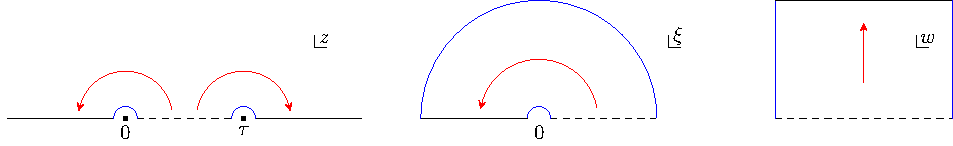
\includegraphics[width=\columnwidth]{fig_H-tau_fold}
\caption{Left: Diagram of Loschmidt echo that reduces to a partition function, where imaginary time is the horizontal direction, the dashed (solid) lines are open (gluing) boundary conditions. Red arrows are the directions of Hamiltonian flow that propagates the dashed line boundary state to the solid line boundary state. The blue semi-circles of radius $\epsilon$ are the UV regulators and they are identified as periodic boundaries in the direction perpendicular to the red arrow (equal time slice). Middle: Image of the map $\xi = \frac{z}{\tau - z}$. {\color{red}The two semi-circles have radii $({\tau}/{\epsilon})^{\pm1}$ respectively.}  Right: Image of $w = \ln \xi$. It is a cylinder by identifying the blue lines and the standard radial quantization procedure can be applied. }
\label{fig:H-tau_fold}
\end{figure}

One subtlety of the above description is that the two semi-circles in the center diagrams of Fig.~\ref{fig:fidel-map} and Fig.~\ref{fig:H-tau_fold} are not precisely concentric. This can be resolved by the following observation. There exists conformal mappings from the non-concentric circles to two standard concentric circles of radii $1$ and $R$ ($R>1$) on the $\zeta$ plane. Then the logarithmic map $w = \ln \zeta$ produces a cylinder of width $\ln R$. In fact, the width of the cylinder is a conformal invariant and only depend on the cross ratio of the half annulus. The four intersection points of two standard concentric circles on $\zeta$ plane are $(\pm 1,0)$ and $(\pm R,0)$, whose cross ratio is
\begin{equation}
\eta = \frac{(1 + R)^2}{(1 - R)^2}. 
\end{equation}
Hence the width of the cylinder is $\ln \frac{\sqrt{ \eta } - 1}{\sqrt{ \eta} + 1}$. Since conformal transformation preserves the cross ratio, this is also the result if just plug in the cross ratio of the slightly non-concentric diagrams of Fig.~\ref{fig:fidel-map} and Fig.~\ref{fig:H-tau_fold}. The calculation in Eq.~\eqref{eq:fidel_cyd_width} and Eq.~\eqref{eq:echo_cyd_width} equivalently used the leading order approximation to $\eta$ in the respective geometry and thus get the leading order term in the width of the cylinder. The slight deviation to the precise concentric geometry will only bring $\frac{\epsilon}{L}, \frac{\epsilon}{\tau}$ corrections to the width parameter and will not affect the fidelity and echo exponents. 

Since the fidelity and Loschmidt echo are both square of the amplitude, we should set the width of the cylinder $\beta = 2 \ln L$ or $ 4 \ln \tau$ after obtaining the partition function on it. 

In App.~\ref{app:lambda_12}, we performed the calculation of the general partition function $S_a( \theta_1 ) \rightarrow S_b( \theta_2)$ and its free energy to the leading order of cylinder width $\beta$. A na\"ive application of the result however will lead to an apparent contradiction. One notable example is that when $a = b  = {\rm P}$, the free energy given by App.~\ref{app:lambda_12} is $- \frac{1}{12}\beta$, which should actually be {\it zero} because this is the (regularized) free energy on a plane without any interface. Physically this corresponds to the situation that the boundary condition does not change after joining the two chains. Hence the Loschmidt echo will stay at $1$ and the free energy is $0$. This motivates a shift to the free energy
\begin{equation}
\mathcal{F} = - \ln Z_{ab} ( \beta ) + \frac{1}{12} \beta ,
\end{equation}
where $\frac{1}{12}\beta$ is the value of $ \ln Z_{ab} ( \beta )$ when $a = b = {\rm P}$. A more careful inspection in App.~\ref{app:F_correction} shows the origin of the shift: part of it comes from the outer semi-circles in the middle panel of Fig.~\ref{fig:fidel-map} and Fig.~\ref{fig:H-tau_fold}, and part comes from the non-homogeneous term in the conformation transformation of the stress tensor from annulus to cylinder. 

After incorporating this shift, for the process ($c$ is assumed to be the same as $a$)
\begin{equation}
\label{eq:S_i_S_j}
S_i( \theta_1 ) \rightarrow S_j( \theta_2 ) ,
\end{equation}
the free energy is
\begin{equation}
\mathcal{F}( \beta )  = 
\left\lbrace
\begin{aligned}
  &\frac{1}{2}(|x| - x^2 )\beta  \quad &i = j \\
  &\frac{1}{16}\beta   \quad &i \ne j ,  \\
\end{aligned} \right. \quad x = \frac{\theta_2 - \theta_1}{\pi} .
\end{equation}
We can then set $\beta = 2 \ln L$ and $ 4 \ln t$ (after analytic continuing to real time) to get the fidelity and echo exponent. 

As analyzed in Sec.~\ref{sec:analytic_numerics}, $S_2( \theta)$ interpolates between DD and NN, $S_1( \theta )$ interpolates between DN and ND. In the region accessible to the numerical calculation in the lattice model, we choose the process ${\rm DD} \rightarrow  \lambda$ to verify
\begin{equation}
\label{eq:result_DDDD}
\mathcal{F} = 
\left\lbrace
\begin{aligned}
\frac{1}{8}\ln L  &\quad\text{fidelity}  \\
\frac{1}{4}\ln t   &\quad \text{echo} .  \\
\end{aligned} \right.  
\end{equation}
The same results have already been obtained for $\lambda = {\rm P}$\cite{stephan_logarithmic_2013,stephan_local_2011,vasseur_universal_2014,vasseur_crossover_2013,kennes_universal_2014}. Another process \rev{$\rm{DN} \rightarrow \lambda$} {\iffalse \color{red} in Eq.~\eqref{eq:DNDN}\fi} is used to verify
\begin{equation}
\label{eq:result_DNDN}
\mathcal{F} = 
\left\lbrace
\begin{aligned}
 (x - x^2 )\ln L   &  \quad {\rm fidelity} \\
 2(x - x^2 ) \ln t  & \quad \text{ Loschmidt echo} , \\
\end{aligned} \right. 
\end{equation}
where $\lambda = \tan \theta$ and $x = \frac{\theta}{\pi}$. 

We also use a more artificial process ${\rm P} \rightarrow \lambda$ to check the shift of the curve
\begin{equation}
\label{eq:periodic-case}
\mathcal{F} = 
\left\lbrace
\begin{aligned}
  \Big(|x-\frac{1}{4}| - (x-\frac{1}{4})^2 \Big)\ln L   &  \quad {\rm fidelity} \\
  2\Big(|x-\frac{1}{4}| - (x-\frac{1}{4})^2 \Big) \ln t  & \quad \text{ Loschmidt echo} .\\
\end{aligned} \right. 
\end{equation}



%%% Local Variables:
%%% TeX-master: "bCFT_paper"
%%% TeX-PDF-mode: t
%%% End:
